%CPET and Jaundice

\chapter{An investigation into the relationship between obstructive jaundice and preoperative pathophysiology in patients undergoing major pancreatic surgery.}

\label{ch_cpet_jaundice}

\lhead{Chapter \ref{ch_cpet_jaundice}. \emph{Obstructive Jaundice}} % This is for the header on each page - perhaps a shortened title

\clearpage

%----------------------------------------------------------------------------------------

\section{Introduction}
Patients with tumours involving the pancreatic head or the periampullary region often present with inoperable disease. In the minority of patients with operable disease, resectional surgery in the form of a pancreaticoduodenectomy remains the main modality of treatment and only chance of a potential cure. However, major pancreatic surgery is associated with significant morbidity and mortality and is only undertaken in specialist centres. Patient selection, preoperative optimisation, good surgical technique and improvements in postoperative care have all contributed to a reduction in mortality \parencite{winter_1423_2006} but morbidity remains high. While several technical strategies have been described in recent years to minimise morbidity, these strategies are not necessarily based on a better understanding of the physiological basis of postoperative complications in these patients.

The anatomical relationship between the distal bile duct, distal pancreatic duct, head of the pancreas and the duodenum is responsible for obstructive jaundice being the most common presenting symptom in patients with tumours affecting this region. Distal bile duct strictures also occur in a small proportion of patients with severe chronic pancreatitis involving the pancreatic head. The perioperative management of the patient with obstructive jaundice is complex and management algorithms are still evolving. 

Obstructive jaundice has been reported to be associated with abnormal cardiovascular physiology in several animal and human studies. Surgery in the jaundiced patient has been reported to be associated with adverse postoperative haemodynamic events and renal dysfunction \parencite{pain_perioperative_1985,green_systemic_1995}. The association between jaundice and cardiovascular physiology was reported over a hundred years ago by King and co-workers who found that injection of porcine bile pigment into dogs resulted in bradycardia, hypotension and eventually death \parencite{king_effect_1909}. Green and co-workers (1986) described the effects of ‘cholemia' in dogs that were subjected to choledochocaval anastomosis. The resultant myocardial depression was described by them as the ‘jaundiced heart'\parencite{green_jaundiced_1986} and has been reported to be associated with poor myocardial response to inotropic stimulation in dogs \parencite{binah_obstructive_1985, bomzon_systemic_1986} as well as humans \parencite{lumlertgul_jaundiced_1991}.

Preoperative biliary drainage used to be advocated before subjecting a patient to pancreaticoduodenectomy with the intention of reducing postoperative morbidity. However, several recent studies have reported that routine PBD is associated with increased complication rates as a consequence of the drainage procedure itself as well as increased incidence of postoperative complications. The DROP trial reported that PBD was associated with drainage related complication as well as postoperative infectious complications. However, this trial excluded patients with a bilirubin levels greater than 250 mg/dl from the study. 

We have recently reported that poor performance at cardiopulmonary exercise testing (CPET) was associated with adverse outcomes after pancreaticoduodenectomy resulting in an increased incidence of POPF and prolonged hospital stay. However, the effects of 'severe jaundice' where bilirubin levels exceed 250 on preoperative patient physiology have not been studied adequately. 

The aim of the present study was to evaluate the relationship between obstructive jaundice and preoperative pathophysiology including cardiopulmonary exercise physiology in patients undergoing pancreaticoduodenectomy.

\clearpage

\section{Patients and Methods}
Patients who underwent classical or pylorus-preserving pancreaticoduodenectomy for periampullary lesions (both benign and malignant) between August 2008 and April 2013 and had undergone cardiopulmonary exercise testing as part of their preoperative work-up at the West of Scotland Pancreatic Unit, Glasgow Royal Infirmary, Glasgow were included in the study. Established criteria for resectability in patients with malignant disease were used as outlined in previous published work. Segmental or wedge resection of the portal vein or superior mesenteric vein was carried out if the lesion was otherwise resectable.

\subsection{Preoperative Data}
Patient demographics, preoperative clinico-pathological characteristics including cardiorespiratory comorbidity, results of preoperative blood tests, chest x-ray, ECG and cardiopulmonary exercise tests were collected from prospectively held databases. The POSSUM Physiology Score was calculated based on 11 physiological parameters (cardiac disease, respiratory disease, ECG changes, pulse rate, blood pressure, haemoglobin, white cell count, serum sodium, serum potassium, serum urea and Glasgow Coma Scale) and was used as an objective score of comorbidity. Cardiovascular comorbidity was defined as a score of 2 or more for either the cardiac disease or ECG component of the POSSUM score. Respiratory comorbidity was defined as a score or 2 or more for the respiratory disease component of the POSSUM score. 

\subsection{Obstructive Jaundice}
Serum bilirubin levels were measured in all patients on the day before surgery. Obstructive jaundice was defined as bilirubin levels greater than 35 micromol/litre and severe obstructive jaundice was defined as bilirubin levels greater than 250 micromol/litre. This threshold was selected because the DROP trial did not investigate patients with bilirubin levels greater than 250 micromol/litre and this study aimed to evaluate preoperative pathophysiology in this particular group. 
\todo{A word about stents}

\subsection{Cardiopulmonary Exercise Test}
Cardiopulmonary exercise tests were performed in the Department of Respiratory Medicine at the Glasgow Royal Infirmary using the ZAN-600 CPET suite (nSpire Health, Longmont, CO 80501, USA) (9). All patients underwent standard pulmonary function tests and spirometry prior to cardiopulmonary exercise testing. A cycle ergometer was used to perform a symptom-limited, incremental work-load test preceded by a 3-minute rest period. The test was stopped when patients achieved their maximum exercise tolerance, when significant ischaemic changes occurred on ECG or for other safety reasons. Peak oxygen consumption achieved at this stage was defined as $\dot{V}_{O_2}$Peak. The $\dot{V}_{O_2}$AT was calculated using the V-slope \parencite{beaver_new_1986,sue_metabolic_1988} and ventilatory equivalents \parencite{society_ats/accp_2003} methods. $\dot{V}_{O_2}$AT less than 10 ml/kg/min was considered to be low based on previous work by us (Chapter \ref{ch_cpet_outcomes}) as well as Ausania and co-workers \parencite{ausania_effects_2012} which has shown increased incidence of complications in these patients. Oxygen consumption at peak exercise ($\dot{V}_{O_2}$Peak) was dichotomised using a cut-off of 16 ml/kg/min. Detailed description of cardiopulmonary exercise testing as well as the physiological parameters described in this study are published elsewhere \parencite{balady_clinicians_2010}.

\subsection{Statistics}
Grouping of the variables was carried out using standard or previously published thresholds. In the absence of such thresholds, the variables were treated as continuous variables. Non-parametric tests were used to analyse the association between categorical and continuous variables while Chi-square tests were used to analyse the association between categorical variables. Univariate and multivariate binary logistic regression analysis was used to study the relationship between preoperative patient characteristics and $\dot{V}_{O_2}$AT / $\dot{V}_{O_2}$Peak. SPSS software (Version 17.0; SPSS Inc., Chicago, IL, USA) was used to perform statistical analysis.

\clearpage

\section{Results}
One-hundred and thirty eight patients underwent pancreaticoduodenectomy with preoperative cardiopulmonary exercise testing during the study period. Over half of the patients were male (n=93, 67\%). Approximately half the number of patients were over the age of 65 (n=68, 49\%) and overweight or obese (n=69, 50\%). Cardiovascular comorbidity was present in 58 patients (42\%) and respiratory comorbidity was present in 12 patients (9\%). Fifty patients (36\%) had a history of cigarette smoking. The POSSUM Physiology Score was greater than 14 in 61 patients (44\%). Obstructive jaundice (serum bilirubin 35 – 250) was present in 32 (23\%) patients while severe obstructive jaundice (serum bilirubin $>$ 250) was present in 19 (14\%) patients. 

The baseline demographic and clinical characteristics of non-jaundiced and jaundiced patients are shown in Table \ref{table:cpet_oj_patient}. A greater proportion of jaundiced patients were females compared to the non-jaundiced cohort (p=0.028) and smokers (p=0.038). Elevated POSSUM Physiology Score (p=0.004) and malignancy (p$<$0.001) were significantly associated with the presence of jaundice. However, there was no statistically significant difference in age, body mass index, cardiovascular comorbidity, respiratory comorbidity or preoperative biliary drainage between the non-jaundiced and jaundiced patients.

%OJ - PREOP CHARACTERISTICS
\begin{table}[p]
\caption{The relationship  between obstructive jaundice and preoperative patient characteristics in patients undergoing pancreaticoduodenectomy.}
\label{table:cpet_oj_patient}
\centering\renewcommand{\arraystretch}{1.4} %Increases space between rows
\setlength{\tabcolsep}{10pt} %sets the space between columns
	\begin{tabular}{| l | c c c c c |}
		\hline
		                             & \multicolumn{5}{c|}{Preoperative Serum Bilirubin ($\mu$mol/L)} \\
		n = 138                      & $\leq$ 17 & 18-35 & 35-250 & $>$ 250 & \textit{p}              \\ \hline
		Age ($\leq$65/$>$65 years)   & 32/33     & 13/9  & 16/16  & 9/10    & 0.935                   \\
		Sex (Male/Female)            & 48/17     & 14/8  & 22/10  & 9/10    & 0.028                   \\
		BMI (Normal/Overweight)      & 30/35     & 12/10 & 20/12  & 7/12    & 0.82                    \\
		Smoking (No / Yes)           & 48/17     & 12/10 & 18/14  & 10/9    & 0.038                   \\
		PPS ($\leq$14/$>$14)         & 39/22     & 16/5  & 9/23   & 8/11    & 0.004                   \\
		Cardiac disease (No/Yes)     & 35/28     & 13/9  & 17/15  & 13/6    & 0.539                   \\
		Respiratory disease (No/Yes) & 57/6      & 20/2  & 29/3   & 18/1    & 0.664                   \\
		Biliary Stent (No/Yes)       & 29/20     & 3/12  & 6/17   & 18/0    & 0.201                   \\
		Cancer (No/Yes)              & 26/39     & 3/19  & 3/29   & 0/19    & $<$0.001                \\ \hline
		\multicolumn{6}{l}{\textit{p} - Chi-square test}
	\end{tabular}
	\medskip
	\caption*{Obstructive jaundice was more common in females, smokers, patients with elevated POSSUM Physiology Score (PPS) and in patients with cancer. BMI - Body Mass Index, PPS - POSSUM Physiology Score}
\end{table}

The relationship between obstructive jaundice and preoperative blood tests is shown in Table \ref{table:cpet_oj_bloods}. Obstructive jaundice was associated with the presence of a systemic inflammatory response as characterised by raised serum C-reactive protein levels and decrease in serum albumin levels (p$<$0.001). The degree of systemic inflammation was proportionate to the severity of jaundice. Non-jaundiced patients had a median CRP of 3.6 mg/dl (inter-quartile range 0.3 - 89) and serum albumin of 37 g/dl (IQR 18 - 46) while patients with severe obstructive jaundice had a median CRP of 13 (IQR 1.7 - 51) and a median serum albumin of 25 g/dl (IQR 18 - 33). Obstructive jaundice was also associated with electrolyte abnormalities including serum sodium, serum potassium and serum chloride levels. Jaundiced patients were more likely to be anaemic (p$<$0.001) with lower haematocrit (p$<$0.001) and lower mean corpuscular volume (p=0.001). However, there was no significant difference in the preoperative renal function, prothrombin time and white cell count between jaundiced and non-jaundiced patients. 

%Table 2
	\begin{sidewaystable}[p]
		\caption{The relationship  between obstructive jaundice and preoperative biochemical parameters in patients undergoing pancreaticoduodenectomy. }
		\label{table:cpet_oj_bloods}
		\centering
		\renewcommand{\arraystretch}{1.4} %Increases space between rows
		\setlength{\tabcolsep}{9pt} %sets the space between columns
		
		\begin{tabular}{| l | c c c c c|}
			\hline
			                           &                   \multicolumn{4}{c}{Preoperative Serum Bilirubin}  &                 \\
			                           & $\leq$ 17        & 18-35            & 35-250           & $>$ 250          & \textit{p}       \\ \hline
			Haemoglobin                & 13.0 (12.1-14.1) & 13.2 (12.5-14.2) & 11.9 (11.1-12.4) & 11.7 (11.3-12.5) & $<$0.001 \\
			Haematocrit                & 0.39 (0.37-0.42) & 0.4 (0.38-0.43)  & 0.35 (0.34-0.37) & 0.36 (0.34-0.37) & $<$0.001 \\
			Mean Corpuscular Volume    & 90.1 (86.8-93.7) & 93.9 (91.1-96.7) & 92.9 (87.9-96.7) & 87.9 (83.5-91.3) & 0.001    \\
			White cell count           & 7.6 (6.5-9.2)    & 7.6 (6.4-9.5)    & 8.2 (6.7-9.4)    & 7.0 (6.2-9.2)    & 0.591    \\
			Prothrombin time           & 11 (10-12)       & 11 (11-12)       & 11 (11-12)       & 11 (11-12)       & 0.618    \\
			Serum Urea                 & 5.0 (4.3-6.1)    & 5.2 (4.0-5.6)    & 5.5 (4.5-6.6)    & 4.5 (2.3-5.3)    & 0.093    \\
			Serum Creatinine           & 71 (64-80)       & 75 (62-94)       & 71 (62-80)       & 65 (53-72)       & 0.221    \\
			Serum Sodium               & 138 (136-140)    & 138 (136-139)    & 138 (135-140)    & 135 (130-137)    & 0.001    \\
			Serum Potassium            & 4.1 (3.9-4.5)    & 4.3 (4.1-4.5)    & 4.1 (3.75-4.25)  & 3.8 (3.6-4)      & $<$0.001 \\
			Serum Chloride             & 104 (102-106)    & 104 (101-106)    & 104 (99.5-106)   & 99 (93-103)      & 0.002    \\
			Aspartate transaminase     & 21 (17-30)       & 29 (27-48)       & 68.5 (33-144)    & 92.5 (70-116)    & $<$0.001 \\
			Alanine transaminase       & 25 (16-41)       & 31 (24-73)       & 86.5 (50-157.5)  & 95 (53-149)      & $<$0.001 \\
			Gamma-glutamyl transferase & 81 (35-267)      & 111 (56-402)     & 263 (107-947)    & 495 (150-951)    & $<$0.001 \\
			Alkaline phosphatase       & 110 (80-149)     & 150 (115-292)    & 233 (174-698.5)  & 372 (272-551)    & $<$0.001 \\
			C-reactive protein         & 3.6 (1.8-9.5)    & 4.3 (2.4-8)      & 6.9 (3.6-33.5)   & 13 (8.3-20)      & $<$0.001 \\
			Albumin                    & 37 (34-39)       & 36 (33-38)       & 31 (28-33)       & 25 (23-28)       & $<$0.001 \\ \hline
			\multicolumn{6}{l}{Values are median (inter-quartile range); \textit{p} - Kruskal-Wallis test}
		\end{tabular}
	\end{sidewaystable}
	
	


Pulmonary function tests including forced vital capacity (FVC), forced expiratory volume in one second (FEV1) and their derived parameters (predicted FEV1, FEV1/FVC, predicted FEV1/FVC) were compared between jaundiced and non-jaundiced patients. There was a trend towards lower forced vital capacity with increasing severity of jaundice but this did not reach statistical significance (p=0.092). There was no association between the other pulmonary function tests and jaundice. (Table \ref{table:cpet_oj_pft}).

%OJ - PFT
\begin{sidewaystable}[p]
	\caption{The relationship  between obstructive jaundice and pulmonary function tests in patients undergoing pancreaticoduodenectomy.}
	\label{table:cpet_oj_pft}
	\centering
	\renewcommand{\arraystretch}{1.4} %Increases space between rows
	\setlength{\tabcolsep}{9pt} %sets the space between columns
	
	\begin{tabular}{|l| c c c c|c|}
		\hline
		                    &              \multicolumn{4}{c|}{Preoperative Serum Bilirubin}              &  \\
		                    & $\leq$ 17        & 18-35            & 35-250            & $>$ 250          & \textit{p} \\ \hline
		FVC                 & 4.09 (3.49-4.69) & 3.76 (3.38-4.59) & 3.76 (3.16-4.05)  & 3.35 (2.85-4.38) & 0.092      \\
		FEV1                & 2.95 (2.39-3.51) & 2.90 (2.12-3.34) & 2.68 (2.37-3.07)  & 2.72 (2.2-3.28)  & 0.556      \\
		PREDICTED FEV1 (\%) & 105.0 (91-116)   & 98.50 (87-114)   & 103.0 (95-111.5)  & 101.0 (94-116)   & 0.761      \\
		FEV1/FVC            & 72.0 (65-77)     & 73.0 (65-78)     & 75.50 (70.5-79.5) & 78.0 (70-82)     & 0.115      \\
		PREDICTED FEV1/FVC  & 94.0 (87-102)    & 96.0 (86-100)    & 99.0 (93-103)     & 102.0 (88-108)   & 0.107      \\ \hline
		\multicolumn{6}{l}{Values are median (inter-quartile range); \textit{p} - Kruskal-Wallis test}
	\end{tabular}
\end{sidewaystable}





Cardiopulmonary exercise test parameters measured at the anaerobic threshold and at peak exercise were compared between jaundiced and non-jaundiced patients using the Kruskal-Wallis test. Obstructive jaundice was associated with lower tidal volume (p=0.017), lower absolute $\dot{V}_{O_2}$ (p=0.003), lower corrected $\dot{V}_{O_2}$ (p=0.029), lower oxygen pulse (p=0.037) and lower respiratory rate (p=0.022). At peak exercise, jaundice was associated with lower tidal volume (p=0.028), lower absolute $\dot{V}_{O_2}$Peak (p=0.007), lower absolute $\dot{V}_{CO_2}$ (p=0.016) and lower end-tidal $O_2$ or $PET_{O_2}$ (p=0.026). However, as shown in Tables \ref{table:cpet_oj_anaerobic} and \ref{table:cpet_oj_peak}, several of these associations were not linear with a trend towards poorer results between non-jaundiced and mildly jaundiced patients and better values in the severely jaundiced cohort. 

%OJ - ANAEROBIC THRESHOLD
\begin{sidewaystable}[p]
	\caption{The relationship  between obstructive jaundice and cardiopulmonary exercise test parameters at the anaerobic threshold in patients undergoing pancreaticoduodenectomy.  }
	\label{table:cpet_oj_anaerobic}
	\centering
	\renewcommand{\arraystretch}{1.2} %Increases space between rows
	%\setlength{\tabcolsep}{9pt} %sets the space between columns
		%6 columns   
	\begin{tabular}{|l| c c c c c|}
		\hline
		                               &             \multicolumn{4}{c}{Preoperative Serum Bilirubin ($\mu$mol/L)}             &  \\
		Anaerobic Threshold            & $\leq$ 17           & 18-35               & 35-250              & $>$ 250             & \textit{p} \\ \hline
		Load  (Watts)                  & 44.3 (32.5-60.0)    & 33.5 (27.5-51.0)    & 41.0 (31.0-56.0)    & 38.3 (30.5-48.0)    & 0.313      \\
		Min. Ventilation (l/min)       & 25.0 (20.4-30.5)    & 23.0 (20.5-29.0)    & 23.0 (19.0-28.0)    & 22.0 (18.5-25.0)    & 0.107      \\
		Tidal Volume (litres)          & 1.26 (1.06-1.52)    & 1.09 (0.83-1.39)    & 1.06 (0.94-1.44)    & 1.08 (0.82-1.26)    & 0.017      \\
		$\dot{V}_{O_2}$ (litres/min)   & 0.85 (0.71-1.00)    & 0.73 (0.62-0.81)    & 0.72 (0.58-0.86)    & 0.70 (0.58-0.82)    & 0.003      \\
		$\dot{V}_{O_2}$/kg (ml/kg/min) & 11.1 (9.8-12.8)     & 10.6 (8.9-11.4)     & 9.9 (8.5-12.7)      & 9.6 (9.3-10.8)      & 0.029      \\
		$\dot{V}_E/\dot{V}_{O_2}$      & 28.5 (25.5-30.1)    & 29.4 (26.7-31.3)    & 28.3 (27.0-34.7)    & 27.8 (24.6-31.9)    & 0.510      \\
		$\dot{V}_{CO_2}$ (litres/min)  & 0.82 (0.66-1.0)     & 0.71 (0.58-0.93)    & 0.75 (0.58-0.90)    & 0.69 (0.52-0.79)    & 0.032      \\
		$\dot{V}_E/\dot{V}_{CO_2}$     & 28.9 (27.2-30.7)    & 28.9 (28.1-30.7)    & 30.6 (26.3-33.1)    & 30.4 (27.9-32.2)    & 0.449      \\
		RER                            & 0.96 (0.9-1.03)     & 0.99 (0.89-1.04)    & 0.98 (0.94-1.07)    & 0.93 (0.91-1.04)    & 0.478      \\
		${PET_O}_2$ (mmHg)             & 110.0 (104.3-112.6) & 113.0 (109.0-115.0) & 111.0 (106.0-117.0) & 111.0 (105.0-114.5) & 0.078      \\
		${PET_{CO}}_2$ (mmHg)          & 36.8 (34.8-39.0)    & 36.0 (34.0-37.5)    & 34.0 (32.0-39.0)    & 35.0 (32.0-39.0)    & 0.204      \\
		$O_2$Pulse (ml/beat)           & 8.0 (7.0-9.0)       & 7.0 (5.0-9.0)       & 7.5 (5.0-9.0)       & 6.7 (5.0-8.0)       & 0.037      \\
		Heart rate (/min)              & 108 (96-122)        & 107 (90-118)        & 101 (89-118)        & 112 (96-125)        & 0.393      \\
		Respiratory Rate (/min)        & 19 (17-21)          & 22 (20-27)          & 21 (18-24)          & 19 (18-23)          & 0.022      \\ \hline
		\multicolumn{6}{l}{Values are median (inter-quartile range); \textit{p} - Kruskal-Wallis test}
	\end{tabular}
	\medskip
	\caption*{At anaerobic threshold, obstructive jaundice was compared to multiple CPET parameters. There were several statistically significant but non-linear relationships between preoperative serum bilirubin and CPET parameters. $\dot{V}_{O_2}$ - Oxygen consumption, $\dot{V}_{CO_2}$ - Exhaled $CO_2$, PET$O_2$/$CO_2$ - Partial pressure of end-tidal $O_2$/$CO_2$, $O_2$Pulse - Oxygen pulse.}
\end{sidewaystable}



%OJ - PEAK EXERCISE
\begin{sidewaystable}[p]
	\caption{The relationship  between obstructive jaundice and cardiopulmonary exercise test parameters at peak exercise in patients undergoing pancreaticoduodenectomy.  }
	\label{table:cpet_oj_peak}
	\centering
	\renewcommand{\arraystretch}{1.4} %Increases space between rows
	%\setlength{\tabcolsep}{9pt} %sets the space between columns
		%6 columns   
	\begin{tabular}{|l| c c c c c|}
		\hline
		                               &               \multicolumn{4}{c}{Preoperative Serum Bilirubin}                &  \\
		Peak Exercise                               & $\leq$ 17         & 18-35             & 35-250            & $>$ 250            & \textit{p} \\ \hline
		Load  (Watts)                  & 94.0 (76.5-114.5) & 87.5 (56.0-107.0) & 73.0 (58.0-108.0) & 85.0 (66.0-101.0)  & 0.066      \\
		Min. Ventilation (l/min)       & 53.5 (46.0-69.0)  & 46.5 (34.0-62.0)  & 46.0 (38.0-63.0)  & 48.0 (37.0-67.0)   & 0.088      \\
		Tidal Volume (litres)          & 1.95 (1.6-2.41)   & 1.64 (1.46-1.98)  & 1.62 (1.35-2.19)  & 1.86 (1.18-2.21)   & 0.028      \\
		$\dot{V}_{O_2}$ (litres/min)   & 1.33 (1.09-1.57)  & 1.14 (0.90-1.32)  & 1.08 (0.85-1.5)   & 1.11 (0.89-1.38)   & 0.007      \\
		$\dot{V}_{O_2}$/kg (ml/kg/min) & 17.2 (14.45-22.0) & 14.7 (13.5-17.3)  & 15.1 (12.7-19.9)  & 15.7 (13.3-19.2)   & 0.056      \\
		$\dot{V}_E/\dot{V}_{O_2}$      & 40.5 (36.2-46.8)  & 43.1 (37.3-46.5)  & 41.9 (38.9-47.4)  & 46.7 (42.1-55.2)   & 0.073      \\
		$\dot{V}_{CO_2}$ (litres/min)  & 1.67 (1.37-2.01)  & 1.32 (1.02-1.84)  & 1.29 (1.04-1.88)  & 1.47 (1.03-1.76)   & 0.016      \\
		$\dot{V}_E/\dot{V}_{CO_2}$     & 31.9 (29.5-34.9)  & 32.1 (29.4-36.4)  & 33.1 (30.2-37.8)  & 37.4 (30.9-40.8)   & 0.110      \\
		RER                            & 1.28 (1.20-1.42)  & 1.27 (1.20-1.42)  & 1.28 (1.22-1.36)  & 1.36 (1.25-1.42)   & 0.675      \\
		${PET_O}_2$                    & 121 (118.5-125)   & 122 (120-126)     & 122 (120-125)     & 126 (123-128)      & 0.026      \\
		${PET_{CO}}_2$                 & 35 (32.5-38)      & 35 (32-38)        & 34 (30-38)        & 33 (29-36)         & 0.283      \\
		$O_2$Pulse                     & 11.9 (9.11-14)    & 10.0 (8.0-12.0)   & 11.0 (9.61-13.93) & 11.65 (8.26-13.94) & 0.132      \\
		Heart rate                     & 140 (125-158)     & 140 (129-152)     & 129 (114-144)     & 134 (128-158)      & 0.158      \\
		Respiratory Rate               & 30 (26-34)        & 32 (28-35)        & 30 (26-34)        & 31 (28-36)         & 0.512      \\
		Exercise Duration (minutes)    & 8.2 (6.2-10.4)    & 6.9 (5.5-9.2)     & 6.6 (4.8-9.0)     & 8.2 (5.2-9.7)      & 0.164      \\ \hline
		\multicolumn{6}{l}{Values are median (inter-quartile range); \textit{p} - Kruskal-Wallis test}
	\end{tabular}
\end{sidewaystable}


Binary logistic regression analysis was undertaken to assess preoperative clinico-pathological patient factors associated with a low $\dot{V}_{O_2}$AT and low $\dot{V}_{O_2}$Peak. On univariate analysis, female sex (HR 2.74, 95\% CI 1.30-5.74, p=0.008), body mass index $>$ 25 (HR 3.09, 95\% CI 1.51-6.32, p=0.002), presence of malignancy (HR 3.59, 95\% CI 1.36-9.43, p=0.010), POSSUM Physiology Score $>$ 14 (HR 2.06, 95\% CI 1.02-4.17, p= 0.044), serum bilirubin $>$ 250 $\mu$mol/l (HR 5.66, 95\% CI 1.87-17.16, p=0.002), haemoglobin $<$ 12 g/dl (HR 2.74, 95\% CI 1.30-5.74, p=0.008) and serum C-reactive protein $>$ 10 mg/dl (HR 2.18, 95\% CI 1.06-4.51, p=0.035) were associated with $\dot{V}_{O_2}$AT $<$ 10 ml/kg/min. Age, cardiovascular and respiratory comorbidity, preoperative biliary drainage, mild jaundice and serum albumin were not significantly related to a low $\dot{V}_{O_2}$AT. 

The statistically significant independent variables with p$<$0.05 were entered into a backward step-wise regression model with $\dot{V}_{O_2}$AT $<$ 10 ml/kg/min as a categorical, binomial, dependent variable. Female sex (HR 3.75, 95\% CI 1.57-8.95 p$<$0.005), body mass index $>$ 25 (HR 3.65, 95\% CI 1.61-8.26, p$<$0.005), malignancy (HR 4.02, 95\% CI 1.33-12.16, p$<$0.05) and C-reactive protein $>$ 10 mg/dl (HR 2.98, 95\% CI 1.29-6.86, p$<$0.05) were independently related to low $\dot{V}_{O_2}$AT. Obstructive jaundice was not related to low $\dot{V}_{O_2}$AT on multivariate analysis. (Table \ref{table:cpet_oj_at_regression})

Binary logistic regression analysis of the relationship between patient factors and low $\dot{V}_{O_2}$Peak ($<$ 16 ml/kg/min) is shown in Table \ref{table:cpet_oj_peak_regression}. On both univariate and multivariate analysis, female sex, body mass index $>$ 25 and haemoglobin $<$ 12 g/dl were significantly associated with a low $\dot{V}_{O_2}$Peak. 

\begin{sidewaystable}[p]
	\caption{The relationship between clinico-pathological characteristics and low $\dot{V}_{O_2}$AT ($<$ 10 ml/kg/min) in patients undergoing pancreaticoduodenectomy: Univariate and multivariate binary logistic regression analysis}
	\label{table:cpet_oj_at_regression}
	\setlength{\tabcolsep}{9pt} %sets the space between columns
	\centering
	\begin{tabular}{|l l c| c c c| c c c|}
		\hline
		Variable                   &           & n   & HR   & 95\% CI    & \textit{p} & HR   & 95\% CI    & \textit{p} \\ \hline
		Age (years)                & $\leq$ 65 & 70  &      &            &            &      &            &  \\
		                           & $>$ 65    & 68  & 1.19 & 0.60-2.35  & 0.628      &      &            &  \\
		Sex                        & Male      & 95  &      &            &            &      &            &  \\
		                           & Female    & 43  & 2.74 & 1.30-5.74  & 0.008      & 3.75 & 1.57-8.95  & 0.003      \\
		Body Mass Index ($kg/m^2$) & $\leq$ 25 & 69  &      &            &            &      &            &  \\
		                           & $>$ 25    & 69  & 3.09 & 1.51-6.32  & 0.002      & 3.65 & 1.61-8.26  & 0.002      \\
		Smoking                    & No        & 88  &      &            &            &      &            &  \\
		                           & Yes       & 50  & 1.38 & 0.68-2.79  & 0.378      &      &            &  \\
		Cardiovascular disease     & No        & 78  &      &            &            &      &            &  \\
		                           & Yes       & 58  & 0.82 & 0.41-1.64  & 0.569      &      &            &  \\
		Respiratory disease        & No        & 124 &      &            &            &      &            &  \\
		                           & Yes       & 12  & 2.37 & 0.71-7.91  & 0.159      &      &            &  \\
		Cancer                     & No        & 32  &      &            &            &      &            &  \\
		                           & Yes       & 106 & 3.59 & 1.36-9.43  & 0.010      & 4.02 & 1.33-12.16 & 0.014      \\
		POSSUM Physiology Score    & $\leq$ 14 & 72  &      &            &            &      &            &  \\
		                           & $>$ 14    & 61  & 2.06 & 1.02-4.17  & 0.044      &      &            & 0.164      \\
		Biliary stent              & No        & 56  &      &            &            &      &            &  \\
		                           & Yes       & 49  & 0.69 & 0.32-1.50  & 0.347      &      &            &  \\
		Bilirubin ($\mu$mol/l)     & $\leq$ 17 & 65  &      &            &            &      &            &  \\
		                           & 18-35     & 22  & 1.49 & 0.54-4.16  & 0.444      &      &            & 0.911      \\
		                           & 36-250    & 32  & 2.30 & 0.95-5.56  & 0.064      &      &            & 0.537      \\
		                           & $>$ 250   & 19  & 5.66 & 1.87-17.16 & 0.002      &      &            & 0.443      \\
		Haemoglobin (g/dl)         & $\geq$ 12 & 95  &      &            &            &      &            &  \\
		                           & $<$ 12    & 43  & 2.74 & 1.30-5.74  & 0.008      &      &            & 0.214      \\
		C-reactive protein (mg/l)  & $\leq$ 10 & 90  &      &            &            &      &            &  \\
		                           & $>$ 10    & 46  & 2.18 & 1.06-4.51  & 0.035      & 2.98 & 1.29-6.86  & 0.010      \\
		Albumin (g/l)              & $\geq$ 35 & 65  &      &            &            &      &            &  \\
		                           & $<$ 35    & 73  & 1.53 & 0.76-3.05  & 0.231      &      &            &  \\ \hline
	\end{tabular}
	\medskip
	\caption*{Impaired oxygen consumption at the anaerobic threshold ($\dot{V}_{O_2}$AT $<$ 10 ml/kg/min) was independently associated with female sex, body mass index $>$ 25 $kg/m^2$, presence of cancer and raised preoperative C-reactive protein (CRP) level ($>$ 10mg/l).}
\end{sidewaystable}
\begin{sidewaystable}[p]
	\caption{The relationship between clinico-pathological characteristics and low $\dot{V}_{O_2}$Peak ($<$ 16 ml/kg/min) in patients undergoing pancreaticoduodenectomy: Univariate and multivariate binary logistic regression analysis}
	\label{table:cpet_oj_peak_regression}
	\setlength{\tabcolsep}{9pt} %sets the space between columns
	\centering
	\begin{tabular}{|l l c| c c c| c c c|}
		\hline
		Variable                   &           & n   & HR   & 95\% CI   & \textit{p} & HR   & 95\% CI   & \textit{p} \\ \hline
		Age (years)                & $\leq$ 65 & 70  &      &           &            &      &           &  \\
		                           & $>$ 65    & 68  & 1.50 & 0.77-2.94 & 0.237      &      &           &  \\
		Sex                        & Male      & 95  &      &           &            &      &           &  \\
		                           & Female    & 43  & 7.44 & 3.18-17.4 & $<$0.001   & 7.57 & 3.09-18.5 & $<$0.001   \\
		Body Mass Index ($kg/m^2$) & $\leq$ 25 & 69  &      &           &            &      &           &  \\
		                           & $>$ 25    & 69  & 2.02 & 1.03-3.99 & 0.042      & 2.57 & 1.18-5.63 & 0.018      \\
		Smoking                    & No        & 88  &      &           &            &      &           &  \\
		                           & Yes       & 50  & 1.90 & 0.94-3.85 & 0.073      &      &           &  \\
		Cardiovascular disease     & No        & 78  &      &           &            &      &           &  \\
		                           & Yes       & 58  & 1.68 & 0.85-3.33 & 0.139      &      &           &  \\
		Respiratory disease        & No        & 124 &      &           &            &      &           &  \\
		                           & Yes       & 12  & 2.35 & 0.67-8.21 & 0.181      &      &           &  \\
		Cancer                     & No        & 32  &      &           &            &      &           &  \\
		                           & Yes       & 106 & 2.06 & 0.90-4.69 & 0.085      &      &           &  \\
		POSSUM Physiology Score    & $\leq$ 14 & 72  &      &           &            &      &           &  \\
		                           & $>$ 14    & 61  & 1.76 & 0.89-3.51 & 0.107      &      &           &  \\
		Preop Biliary Drainage     & No        & 56  &      &           &            &      &           &  \\
		                           & Yes       & 49  & 0.91 & 0.42-1.97 & 0.814      &      &           &  \\
		Bilirubin ($\mu$mol/l)     & $\leq$ 17 & 65  &      &           &            &      &           &  \\
		                           & 18-35     & 22  & 2.31 & 0.86-6.19 & 0.096      &      &           &  \\
		                           & 36-250    & 32  & 1.60 & 0.68-3.76 & 0.281      &      &           &  \\
		                           & $>$ 250   & 19  & 2.74 & 0.95-7.90 & 0.062      &      &           &  \\
		Haemoglobin (g/dl)         & $\geq$ 12 & 95  &      &           &            &      &           &  \\
		                           & $<$ 12    & 43  & 2.80 & 1.32-5.93 & 0.007      & 2.43 & 1.05-5.63 & 0.038      \\
		C-reactive protein (mg/l)  & $\leq$ 10 & 90  &      &           &            &      &           &  \\
		                           & $>$ 10    & 46  & 1.42 & 0.69-2.90 & 0.333      &      &           &  \\
		Albumin (g/l)              & $\geq$ 35 & 65  &      &           &            &      &           &  \\
		                           & $<$ 35    & 73  & 1.28 & 0.65-2.49 & 0.476      &      &           &  \\ \hline
	\end{tabular}
	\medskip
	\begin{flushleft}
		Oxygen consumption at peak exercise ($\dot{V}_{O_2}$Peak) $<$ 16 ml/kg/min was independently associated with female sex, body mass index $>$ 25 $kg/m^2$, presence of cancer and raised preoperative C-reactive protein (CRP) level ($>$ 10 mg/l).
	\end{flushleft}
\end{sidewaystable}

\clearpage

Scatter-plot analysis comparing serum bilirubin versus $\dot{V}_{O_2}$AT and $\dot{V}_{O_2}$Peak as continuous variables is depicted in Figure \ref{fig:cpet_oj_scatter}. This shows that the relationship between serum bilirubin and $\dot{V}_{O_2}$AT is weak with a $\rho^2$ value of 0.035 Pearson's $\rho$ = - 0.187, p = 0.028. There was no correlation between serum bilirubin and $\dot{V}_{O_2}$Peak (Pearson's $\rho$ = - 0.132, $\rho^2$ = 0.017, p = 0.123)

\begin{figure}[p]
	\centering
	\begin{subfigure}{0.6\textwidth}
		\centering
		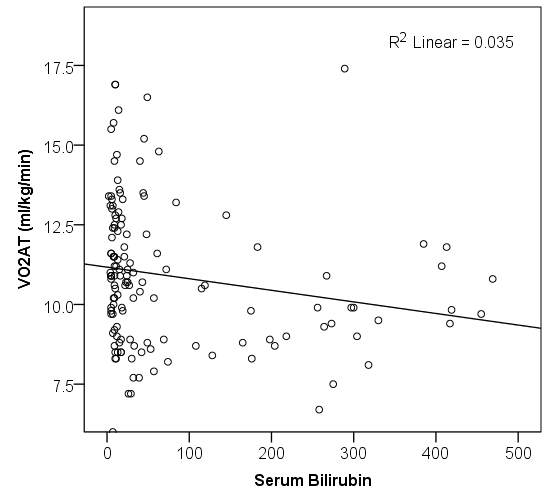
\includegraphics[width=\textwidth]{Figures/cpet_oj_scatter_at_bil}
		\caption{Pearson's $\rho$ = - 0.187, $\rho^2$ = 0.035, p = 0.028}
		\label{fig:cpet_oj_scatter_at_bil}
	\end{subfigure}
	\begin{subfigure}{0.6\textwidth}
		\centering
		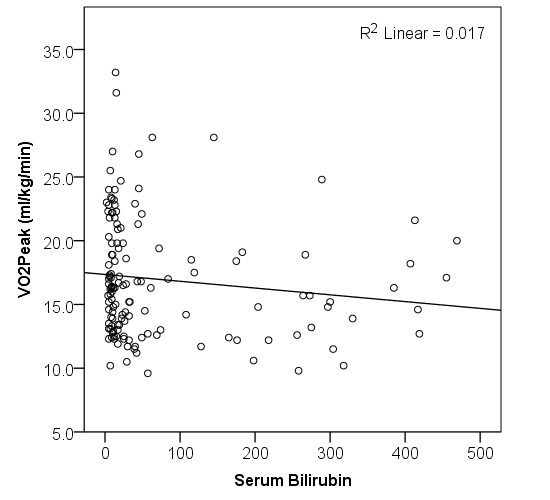
\includegraphics[width=\textwidth]{Figures/cpet_oj_scatter_peak_bil}
		\caption{$\rho$ = - 0.132, $\rho^2$ = 0.017, p = 0.123}
		\label{fig:cpet_oj_scatter_peak_bil}
	\end{subfigure}
	
	\caption{Pearson's correlation and scatter-plot analysis comparing serum bilirubin versus $\dot{V}_{O_2}$AT and $\dot{V}_{O_2}$Peak in patients undergoing pancreaticoduodenectomy.}
	\label{fig:cpet_oj_scatter}
	
\end{figure}


\clearpage

\section{Discussion}
The optimal preoperative management of obstructive jaundice, especially with extremely high serum bilirubin levels, in the patient with periampullary cancer requiring pancreaticoduodenectomy is still unclear. The results of the present study also show for the first time that while obstructive jaundice is associated with a range of biochemical and haematological abnormalities, it does not affect cardiopulmonary physiology as measured by cardiopulmonary exercise testing. 

The use of CPET in preoperative risk prediction was first made popular over two decades ago by Older and co-workers \parencite{older_preoperative_1993}. Since then cardiopulmonary exercise testing has been reported to be useful in identifying high risk patients prior to major general \parencite{snowden_submaximal_2010}, pancreatic \parencite{ausania_effects_2012},[Chapter \ref{ch_cpet_outcomes}], oesophagogastric \parencite{nagamatsu_preoperative_2001} as well as vascular \parencite{carlisle_mid-term_2007} surgery. Cardiopulmonary exercise testing has been reported to be superior to conventional measures of comorbidity chiefly due to the dynamic nature of the test that evaluates the adequacy of oxygen delivery to tissues under physiological stress. However, the factors responsible for poor aerobic capacity in preoperative patients have not been adequately studied.

The association between jaundice and cardiovascular physiology was reported over a hundred years ago by King and co-workers who found that injection of porcine bile pigment into dogs resulted in bradycardia, hypotension and eventually death \parencite{king_effect_1909}.

Jaundice has been reported to be associated with myocardial depression \parencite{green_jaundiced_1986}, poor myocardial response to inotropic stimulation \parencite{lumlertgul_jaundiced_1991}, impaired sympathetic baroreflex sensitivity \parencite{song_baroreflex_2009}, deranged atrial natriuretic peptide levels \parencite{pereira_increased_1994,gallardo_increased_1998} as well as multiple other bile-acid receptor mediated effects on the cardiovascular system \parencite{khurana_bile_2011}. Moreover, some of these effects appear to be partly reversible by biliary drainage as demonstrated by Padillo and coworkers \parencite{padillo_improved_2001}.

Historically, obstructive jaundice has also been reported to be associated with adverse haemodynamic events in patients undergoing major surgery. Intraopertive blood loss, postoperative hypotension, increased susceptibility to shock and renal dysfunction were all more common in patients with obstructive jaundice. This increased incidence of complications as a consequence of obstructive jaundice resulted in routine PBD being recommended in these patients in order to alleviate their jaundice before undertaking major surgery. In fact, Whipple described his earliest pancreaticoduodenectomy as a two-stage operation, with the first stage aimed at performing a biliary bypass to reduce jaundice levels before undertaking the resection at a later second operation.

However, more recently, there has been increasing evidence that such routine PBD may itself be associated with increased complications both associated with the drainage procedure itself as well as the effects of PBD on surgical outcomes.

Pitt and coworkers in a prospective randomised trial comparing outcomes in jaundiced patients undergoing surgery with or without PBD reported that PBD was associated with increased cost without any decrease in postoperative complications \parencite{pitt_does_1985}. But, this study looked at a heterogenous group of patients of which only 7 underwent pancreaticoduodenectomy.

A recent meta-analysis \parencite{sewnath_meta-analysis_2002} analysed data from 5 randomised controlled trials comparing surgery with PBD versus surgery without PBD and concluded that PBD not only did not improve postoperative complication rates or mortality but resulted in a higher overall complication rate due to the morbidity associated with the procedure itself. All five RCTs included in this meta-analysis included a heterogenous group of operations with only a few undergoing pancreaticoduodenectomy while more than 50\% of patients underwent palliative bypass or exploratory laparotomy making comparison of outcomes difficult. A recent Cochrane Collaboration review of six trials including 520 patients concluded that PBD may be associated with serious adverse events and must not be performed routinely outwith trial settings \parencite{wang_preoperative_2008}.

The DROP trial sought to clarify the role of PBD in patients undergoing pancreaticoduodenectomy \parencite{van_der_gaag_preoperative_2010}. It randomised patients with bilirubin levels between 40 and 250 either to undergo surgery without PBD or to undergo PBD followed by surgery after 4 - 6 weeks. The authors reported that PBD resulted in an increase in incidence of complications of which the majority were related to the drainage procedure itself. However, this trial excluded patients with bilirubin levels over 250.

While the aforementioned studies have undermined the role of PBD in jaundiced patients undergoing pancreaticoduodenectomy, the results of the present study show for the first time that the premise for performing PBD, namely the adverse effect of jaundice on cardiopulmonary physiology may itself be flawed in patients undergoing pancreaticoduodenectomy. In our study, obstructive jaundice including severe obstructive jaundice did not affect cardiopulmonary exercise capacity as measured by $\dot{V}_{O_2}$AT or the peak oxygen consumption. These findings taken together with previously published findings of adverse effects of PBD further support the fact that major surgery may be safe in jaundiced patients without subjecting them to preoperative biliary drainage. 
The basis of the relationship between low $\dot{V}_{O_2}$AT and raised BMI is not clear. 

However, such an association has been previously reported \parencite{horwich_relationship_2009}  This may reflect the difficulty in obtaining accurate $\dot{V}_{O_2}$AT values in obese patients as a result of the calculations involved rather than due to true cardiopulmonary dysfunction. Other authors have suggested that different thresholds for CPET parameters may have to be considered in obese patients to improve risk-prediction \parencite{donnelly_criteria_1990,hulens_exercise_2001}. Cardiopulmonary exercise testing measures oxygen delivery to skeletal muscle. Adipose tissue, however, does not contribute to the metabolic activity that is measured during CPET. However, AT as normally reported, is calculated by dividing the oxygen consumption per minute at the ‘anaerobic threshold' into the weight of the patient. However, this does not account for the disproportionately higher amount of adipose tissue in overweight/obese patients resulting in a spuriously low AT (in mls/kg/min). The present study found no association between cardiorespiratory comorbidity and $\dot{V}_{O_2}$AT. Low $\dot{V}_{O_2}$AT in female patients and overweight/obese patients should be interpreted with caution as this may not be due to true poor aerobic capacity.

\section{Conclusions}
Obstructive jaundice, including severe obstructive jaundice (serum bilirubin>250 mg/dl) does not affect preoperative cardiopulmonary exercise physiology. Reduction of cardiovascular adverse events can no longer be the rationale for preoperative biliary drainage even in patients with severe obstructive jaundice. Future studies must evaluate the safety of elective surgery in patients with severe jaundice and show comparable outcomes to non-jaundiced patients before PBD can be completely abandoned except in special circumstances.